%
% CMPT 300: Operating Systems I - A Course Overview
% Section: Processes
%
% Author: Jeffrey Leung
%

\section{Processes}
	\label{sec:processes}
\begin{easylist}

& \textbf{Process:} Program which is loaded in memory and currently being executed (i.e. the required OS structures exist)
	&& Consists of a program counter, stack (which includes local variables and return address), and data location/area (which includes global variables and dynamically allocated memory) (see figure~\ref{fig:processes:process-data})
	\begin{figure}[!htb]
		\centering
		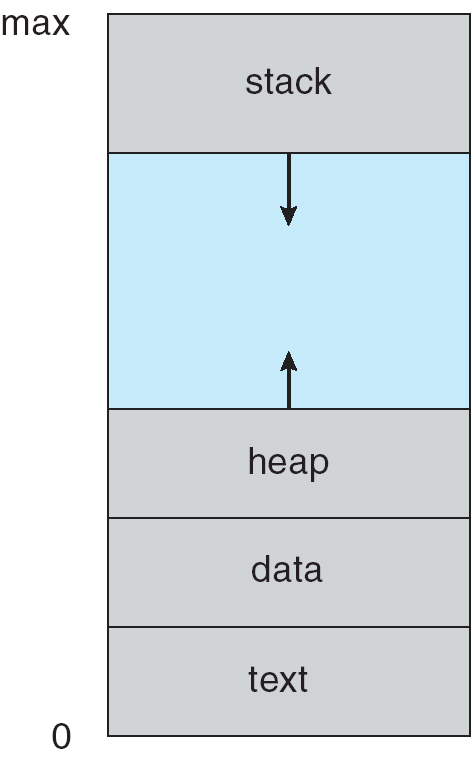
\includegraphics[width=0.3\textwidth]{process-data}
		\caption{Process Data}
		\label{fig:processes:process-data}
	\end{figure}
	&& Created by a parent process; may create children processes

& \textbf{Process state:} Current execution stage of a process
	&& New, running, waiting (for an event), ready (waiting for CPU), terminated
& \textbf{Process Control Block (PCB):} Set of data about a particular process
	&& Used to switch the CPU between processes
	&& Data includes process state, program counter, CPU registers, CPU scheduling information, memory management information, I/O status information

& Managed in scheduling queues
	&& \textbf{Ready queue:} Set of processes in memory which are ready to execute
	&&& \textbf{Device queue:} Set of processes in memory which are waiting for an I/O device
	&& See figure~\ref{fig:processes:scheduling-queues}
	\begin{figure}[!htb]
		\centering
		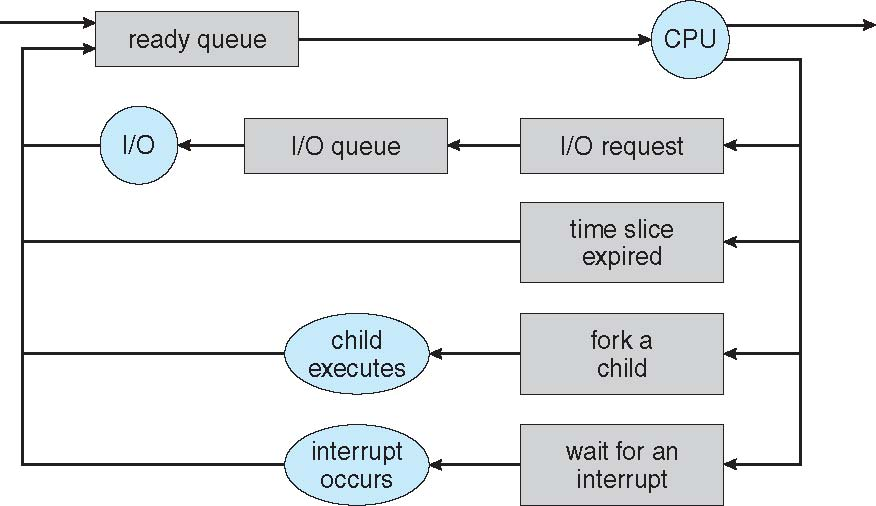
\includegraphics[width=0.7\textwidth]{scheduling-queues}
		\caption{Scheduling Queues}
		\label{fig:processes:scheduling-queues}
	\end{figure}

& \textbf{Context switch:} CPU changing from one process to another
	&& State of the first process is saved in a PCB in memory; state of the second process from another PCB in memory is loaded into the registers
	&& \textbf{CPU state:} Values of the CPU registers
		&&& Includes program counter and stack counter
	&& Overhead with no work done
	&& Usually several milliseconds
	&& Some systems use multiple register sets which can be easily switched between using pointers

&& \textbf{Fork:} System call executed by a process (parent) which creates a new process (child)
	&&& Child is a copy of the parent
	&&& Child loads another program using the \lstinline[columns=fixed]{exec()} system call % [ Left bracket to fix syntax highlighting error by Texmaker
	&&& Parent waits for children to exit, or aborts the execution of its children
		&&&& \textbf{Cascade termination:} Abortion of the children of a child process
		&&&& OS deallocates resources
		&&&& Data is returned to parent via \lstinline[columns=fixed]{wait()} % [ Left bracket to fix syntax highlighting error by Texmaker
		&&&& \textbf{Zombie process:} Process which has been terminated but whose parent has not yet called \lstinline[columns=fixed]{wait()} % [ Left bracket to fix syntax highlighting error by Texmaker
			&&&&& Return value held temporarily in memory
		&&&& \textbf{Orphan process:} Process which is running but its parent has exited (without calling \lstinline[columns=fixed]{wait()}) % [ Left bracket to fix syntax highlighting error by Texmaker
			&&&&& \textbf{Adoption:} Changing the parent of an orphaned process to the \lstinline[columns=fixed]{init} process % [ Left bracket to fix syntax highlighting error by Texmaker

\end{easylist}
\subsection{Threads}
	\label{subsec:processes:threads}
\begin{easylist}

& \textbf{Thread:} Sequence of instructions which the CPU can execute as a unit
	&& Tracked by program counter, register set, and stack
	&& Created by system call \lstinline[columns=fixed]{clone()} % [ Left bracket to fix syntax highlighting error by Texmaker
		&&& Can be parameterized to share or duplicate resources
	&& Equivalent to processes in Linux

& \textbf{Multithreading:} Utilization of multiple threads by a single process
	&& Threads of the same process share a code section, data section, and OS resources
	&& Benefits: Responsive, shares resources, scalable
	&& If \lstinline[columns=fixed]{fork()} is called by a process with multiple threads, all threads are duplicated unless \lstinline[columns=fixed]{exec()} is called immediately afterwards

& \textbf{User-level thread:} Thread operating only in user space
	&& Data structures and thread operations are in user level/mode only
	&& Kernel is not aware of user-level threads
& \textbf{Kernel-level thread:} Thread operating only in kernel space
	&& Data strcutures and thread operations are in kernel level/mode (requiring system calls)
	&& Provided by the kernel

& Mappings from user threads to kernel threads:
	&& One-to-one: User level threads are mapped individually to kernel threads
		&&& Pros: Increased concurrency (multiprocessors can be used); one thread cannot block another
		&&& Con: Significant overhead for thread resource usage and management
	&& Many-to-one: Threads are managed in user level to have several user threads map to a single kernel thread
		&&& Pro: Faster thread management due to no switching or system calls
		&&& Cons: A single thread can block all other threads; incompatible with multiprocessors
		&&& E.g. Solaris Green Threads library
	&& Many-to-many: Multiple user threads are mapped to multiple kernel threads
		&&& \textbf{Thread scheduler:} User-level module which manages mapping of user threads to kernel threads
			&&&& \textbf{Upcall:} Notification by kernel when a user thread blocks so another user thread can use the free kernel thread
				&&&&& Complex processing to redirect other threads, nearly duplicating kernel-level work
			&&&& Pros: Increased concurrency and flexibility
			&&&& Con: Difficult to implement

& E.g. POSIX Pthreads API specification used in UNIX systems
	&& \lstinline[columns=fixed]{pthread_create()} blocks until \lstinline[columns=fixed]{pthread_exit()}
	&& \lstinline[columns=fixed]{pthread_join()} combines the two threads % [ Left bracket to fix syntax highlighting error by Texmaker

& \textbf{Thread pool:} Limited set of user-level threads which are either available for use or in use
	&& Removes the overhead of creating new threads
	&& When a new request is created, an inactive thread is pulled from the pool to service the task
	&& Used commonly in web servers to service incoming requests

\end{easylist}
\subsection{Signals}
	\label{subsec:processes:signals}
\begin{easylist}

& \textbf{Signal:} Event notification sent to a process
	&& \textbf{Synchronous signal:} Signal to the same process which caused the signal
		&&& Specific to the thread which caused the signal
		&&& E.g. Illegal memory access
	&& \textbf{Asynchronous signal:} Signal from one process to another
		&&& Delivered to all threads of the process
		&&& E.g. Cancelling a running process with \lstinline[columns=fixed]{Ctrl-C} % [ Left bracket to fix syntax highlighting error by Texmaker

& \textbf{Signal handler:} OS or user-defined module which processes a signal

& Comparison to \hyperref[sec:introduction]{interrupts} (see figure~\ref{fig:processes:comparison}):

\end{easylist}
\begin{figure}[!htb]
	\centering
	\caption{Comparison between Interrupts and Signals}
	\label{fig:processes:comparison}
	\begin{tabular}{ r | p{6cm} p{6cm} }
		& Interrupts & Signals \\
		\hline
		Initiated by &
		\parbox[t]{5cm}{CPU (e.g. division by 0),\\I/O devices (e.g. user input), or\\software (e.g.system call)} &
		\parbox[t]{5cm}{Kernel (e.g. SIGIO) or\\process (e.g. SIGKILL)} \\
		Handled by &
		Interrupt Service Routine in kernel space &
		\parbox[t]{5cm}{Kernel (default) or\\process (manual override)\\in user space} \\
		Continuation &
		May map to signals and deliver to processes for specific handling &
		May have complex logic to call other functions in kernel
	\end{tabular}
\end{figure}
\begin{easylist}

\end{easylist}
\clearpage